\documentclass[review,preprint,12pt]{elsarticle}
%\biboptions{numbers,super,comma}
\biboptions{round,authoryear,semicolon}
\renewcommand{\cite}{\citep} % make default citations parenthetical

\usepackage{amsmath}
\usepackage{amssymb}
\usepackage{amsthm}

\usepackage{graphicx}
%\usepackage{natbib}
\usepackage{caption}
\usepackage{subcaption}
\usepackage{hyperref}

\usepackage{color}
\usepackage{soul}

\usepackage{diagbox}

% Code from http://tex.stackexchange.com/questions/15735/adding-arrows-to-each-term-of-an-equation
\usepackage{tikz}
\usetikzlibrary{arrows}

\makeatletter

% Define how TiKZ will draw the nodes
\tikzset{mathterm/.style={draw=black,fill=white,rectangle,anchor=base}}
\tikzstyle{every picture}+=[remember picture]
\everymath{\displaystyle}

% Designate a term in a math environment to point to
% Syntax: \mathterm[node label]{some math}
\newcommand\mathterm[2][]{%
   \tikz [baseline] { \node [mathterm] (#1) {$#2$}; }}

% A command to draw an arrow from the current position to a labelled math term
% Default color=black, default arrow head=stealth
% Syntax: \indicate[color]{term to point to}[path options]
\newcommand\indicate[2][black]{%
   \tikz [baseline] \node [inner sep=0pt,anchor=base] (i#2) {\vphantom|};
   \@ifnextchar[{\@indicateopts{#1}{#2}}{\@indicatenoopts{#1}{#2}}}
\def\@indicatenoopts#1#2{%
   {\color{#1} \tikz[overlay] \path[line width=1pt,draw=#1,-stealth] (i#2) edge (#2);}}
\def\@indicateopts#1#2[#3]{%
   {\color{#1} \tikz[overlay] \path[line width=1pt,draw=#1,-stealth] (i#2) [#3] edge (#2);}}

\makeatother

%\biboptions{numbers,super,comma}

\newtheorem{theorem}{Theorem}[section]
\newtheorem{lemma}[theorem]{Lemma}

\theoremstyle{definition}
\newtheorem{definition}[theorem]{Definition}
\newtheorem{example}[theorem]{Example}
\newtheorem{xca}[theorem]{Exercise}

\theoremstyle{remark}
\newtheorem{remark}[theorem]{Remark}

\numberwithin{equation}{section}

%    Absolute value notation
%\newcommand{\abs}[1]{\lvert#1\rvert}

%    Blank box placeholder for figures (to avoid requiring any
%    particular graphics capabilities for printing this document).
\newcommand{\blankbox}[2]{%
  \parbox{\columnwidth}{\centering
%    Set fboxsep to 0 so that the actual size of the box will match the
%    given measurements more closely.
    \setlength{\fboxsep}{0pt}%
    \fbox{\raisebox{0pt}[#2]{\hspace{#1}}}%
  }%
}

\journal{Cell Systems}

\begin{document}

\begin{frontmatter}

\title{ %Exploiting redundancy in biological data to scale search tools with entropy \\
An entropy-scaling data structure for searching large-scale biological data}

%    Information for first author
\author[mitmath,mitcsail]{Y. William Yu\corref{co}}
%\ead{ywy@mit.edu}
\author[mitmath,mitcsail]{Noah M. Daniels\corref{co}}
%\ead{ndaniels@csail.mit.edu}
\author[mitcsail]{David C. Danko}
%\ead{dcdanko@mit.edu}
\author[mitmath,mitcsail]{Bonnie Berger\corref{correspond}}
\ead{bab@mit.edu}
%    Address of record for the research reported here
\cortext[co]{These authors contributed equally to this work.}
\cortext[correspond]{Corresponding author}
\address[mitmath]{Department of Mathematics, Massachusetts Institute of Technology, Cambridge, Massachusetts 02139}
\address[mitcsail]{Computer Science and AI Lab, Massachusetts Institute of Technology, Cambridge, Massachusetts 02139}

%\email{bab@mit.edu}

%    General info
%\subjclass[2010]{Primary 68W99}

%\date{September 23, 2014}

%\dedicatory{This paper is dedicated to our advisors.}

%\begin{keyword}
%Similarity search, approximate matching, entropy scaling algorithms
%\end{keyword}

\begin{abstract}
    \begin{itemize}
        \item Low entropy data sets are common in Biological Big Data problems
        \item Under common structural assumptions, it is possible to construct a data structure admitting similarity search in time- and space-complexity roughly linear to ``entropy''
        \item For problems drawn from genomics, small molecule search, and protein structure search, we demonstrate substantial acceleration of analyses using this data structure
    \end{itemize}
\noindent\unskip\textbf{eTOC Blurb}
\par\medskip\noindent\unskip\ignorespaces
Massive data sets in cell systems often exhibit high redundancy and thus low entropy.
We have developed a data structure for similarity search whose complexity scales with entropy.
This approach allows us to achieve massive acceleration of tools drawn from genomics, small molecule search, and protein structure search.
\end{abstract}

\end{frontmatter}

%\maketitle
\section{Summary}
{ \bfseries
    The continual onslaught of new data from cell systems has forced upon scientists the fortunate problem of having too much data to analyze.
    Luckily, it turns out that many data sets exhibit well-defined structure that can be exploited for the design of 
smarter analysis tools.
    We introduce an entropy-scaling data structure---which given a low fractal dimension guarantee, scales in both time and space with the entropy of the underlying database---to perform similarity search, a fundamental operation in data science.
    Using these ideas, we present accelerated versions of standard tools for use by practitioners in the three domains of metagenomics, high-throughput drug screening, and protein structure search:
    CaBLASTX, 700x speedup of BLASTX with less than 5\% loss in sensitivity and no loss in specificity; Ammolite, \hl{??}x speedup of small molecule similarity search; and, esFragBag, 2-30x speedup of FragBag with less than 0.2\% loss in sensitivity and no loss in specificity.

    Source code: \url{http://gems.csail.mit.edu}
}

\section{Introduction}
Throughout all areas of data science, scientists are being confronted by an 
explosion of data.
In many fields, this increase is exponential in nature, outpacing Moore's and Kryder's laws on the respective doublings of transistors on a chip and long-term data storage density \hl{[cite]}.
As such, the challenges posed by the massive influx of data cannot be solved by waiting for faster and larger capacity computers, but require instead the development of data structures and representations that exploit and simplify complexity in the data set.

Here, we focus our attention on similarity search, where the task at hand is to find all entries in some database that are `similar', or approximate matches, to some query item.
Much like sorting is a primitive operation in computer science, similarity search is a fundamental operation in data science and lies at the heart of many other problems.
Traditionally, approximate matching has been studied primarily in the context of strings under edit distance metrics (e.g., for spell-checkers) \cite{ukkonen1985algorithms}.
However, similarity search has also demonstrated increasing importance in biological system domains, including local alignment of sequences \cite{altschul1990basic, kent2002blat}, chemical graphs \cite{schaeffer2007graph}, and protein structures \cite{budowski2010fragbag}.
%In recent years, however, similarity search has become increasingly important for other objects and distance functions (e.g., biological genomes and alignment scores, networks and the Jaccard index) [Altschul et al, 1990; Kent, 2002; Schaeffer, 2007].

As available data grows exponentially \cite{berger2013computational,yu2015quality} (e.g., genomic data in Figure S2), 
%move figure to supplement
algorithms that scale linearly with the amount of data no longer suffice.
The primary ways the literature addresses this problem (e.g.
locality sensitive hashing \cite{indyk1998approximate}, vector approximation \cite{ferhatosmanoglu2000vector}, space partitioning \cite{weber1998quantitative}) involve the construction of data structures that admit a more efficient search operation.
However, we note that as data increases, very often the redundancy present in the data also increases \cite{loh2012compressive}.
Existing general purpose methods do not explicitly exploit this particular feature of biological data.

In the specific context of local alignment in genomics, however, the emerging field of ``compressive genomics'' has shown that existing tools such as BLAST and BLAT can be ``compressively accelerated'' by taking advantage of high redundancy between related genomes using link pointers and edit scripts to a database of unique sequences \cite{loh2012compressive}.
Similar results have been demonstrated for local alignment in proteomics, using much the same strategies \cite{daniels2013compressive}.
Empirically, this compressive acceleration appears to scale almost linearly in the entropy of the database, often resulting in orders of magnitude better performance.

In this paper, we substantially generalize and formalize this approach by introducing a practical opportunistic data structure for similarity search that \textbf{provably} scales almost linearly in both time and space with the entropy of the database.
Specifically, if similarity is defined by a metric-like distance function (e.g., edit or Hamming distance) and the database exhibits both low `metric entropy' and `fractal dimension' (See Supplemental Methods: Theory), this data structure performs much better than na\"ive and even optimized methods.
This data structure allows for minimal (or even zero) loss in recall, coupled
with zero loss in specificity.
%We will define metric entropy and fractal dimension more precisely later, but intuitively, they are respectively measures of the total information content and scaling behavior of number of points contained in spheres of varying radii.
Although these `entropy-scaling data structures' can in principle be used to organize nearly any large data set for faster and more space-efficient analysis,
we demonstrate their utility on similarity search problems drawn from the three major biological `big challenges of big data': genomics, pharmaceuticals, and protein structure \cite{marx2013biology}.

\section{Results}
\subsection{Entropy-scaling data structure for similarity search}
\begin{figure}[btp]
    \centering
    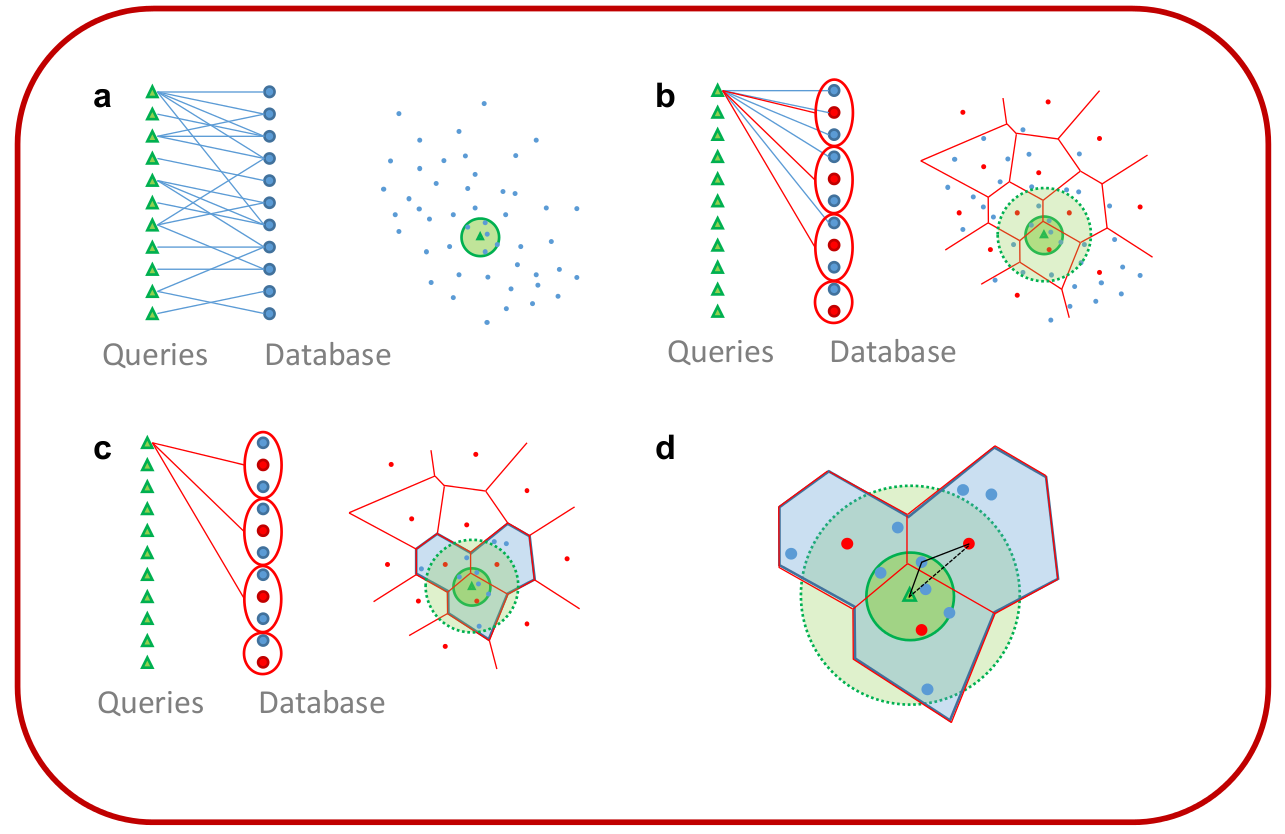
\includegraphics[width=1\textwidth]{assets/dataStructure.png}
    \caption{ Entropy-scaling data structure for similarity search. %
            (a) The na\"ive approach tests each query against each database entry to find entries within distance $X$  of the query. %
            (b) By selecting appropriate cluster centers with maximum radius $r_c$ to partition the database, we can (c) first do a coarse search to find all cluster centers within distance $r+r_c$ of a query, and then the (d) triangle inequality guarantees that a fine search over all corresponding cluster entries will suffice.}
    \label{fig:dataStructure}
\end{figure}

%We present here an opportunistic data structure for similarity search that scales with the entropy of the underlying database.
In the following we consider entropy to be nearly synonymous with distance between points in a high-dimensional space.
For genomic sequences, this can be edit distance, for chemical graphs, maximum common subgraph size, and for general vectors, Euclidean or cosine distance.
The similarity search problem we are most interested in is finding all points in a set that are close to (i.e. similar to) the query point.
The basics of the data structure itself are presented in Figure \ref{fig:dataStructure}, but understanding why it works requires a bit more intuition.

Let's first consider what it means for a large biological data set, considered as points in a high-dimensional space, to be highly redundant.
Perhaps many of the points are exact duplicates; this easy scenario is trivially exploited by de-duplication and is already standard practice (e.g. the NR NCBI protein database \cite{pruitt2005ncbi}).
Or maybe the points mostly live on a low-dimensional subspace; statistical tools such as PCA (Principal Component Analysis) exploit this property in data analysis.
Furthermore, if the dimension of the subspace is sufficiently low,
it can be divided into cells, allowing quick similarity searches by looking only at nearby cells \cite{weber1998quantitative}.
However, when the dimensionality of the subspace increases, cell search time blows up exponentially; additionally, in sparse data sets, most of the cells will be empty, which wastes search time.
%Also, cell search performs poorly when each of the dimensions is small and discrete, as is the case with genomic sequences when we consider each position as a dimension and the four possible nucleotides as the possible locations along that axis.

\begin{figure}[btp]
    \centering
    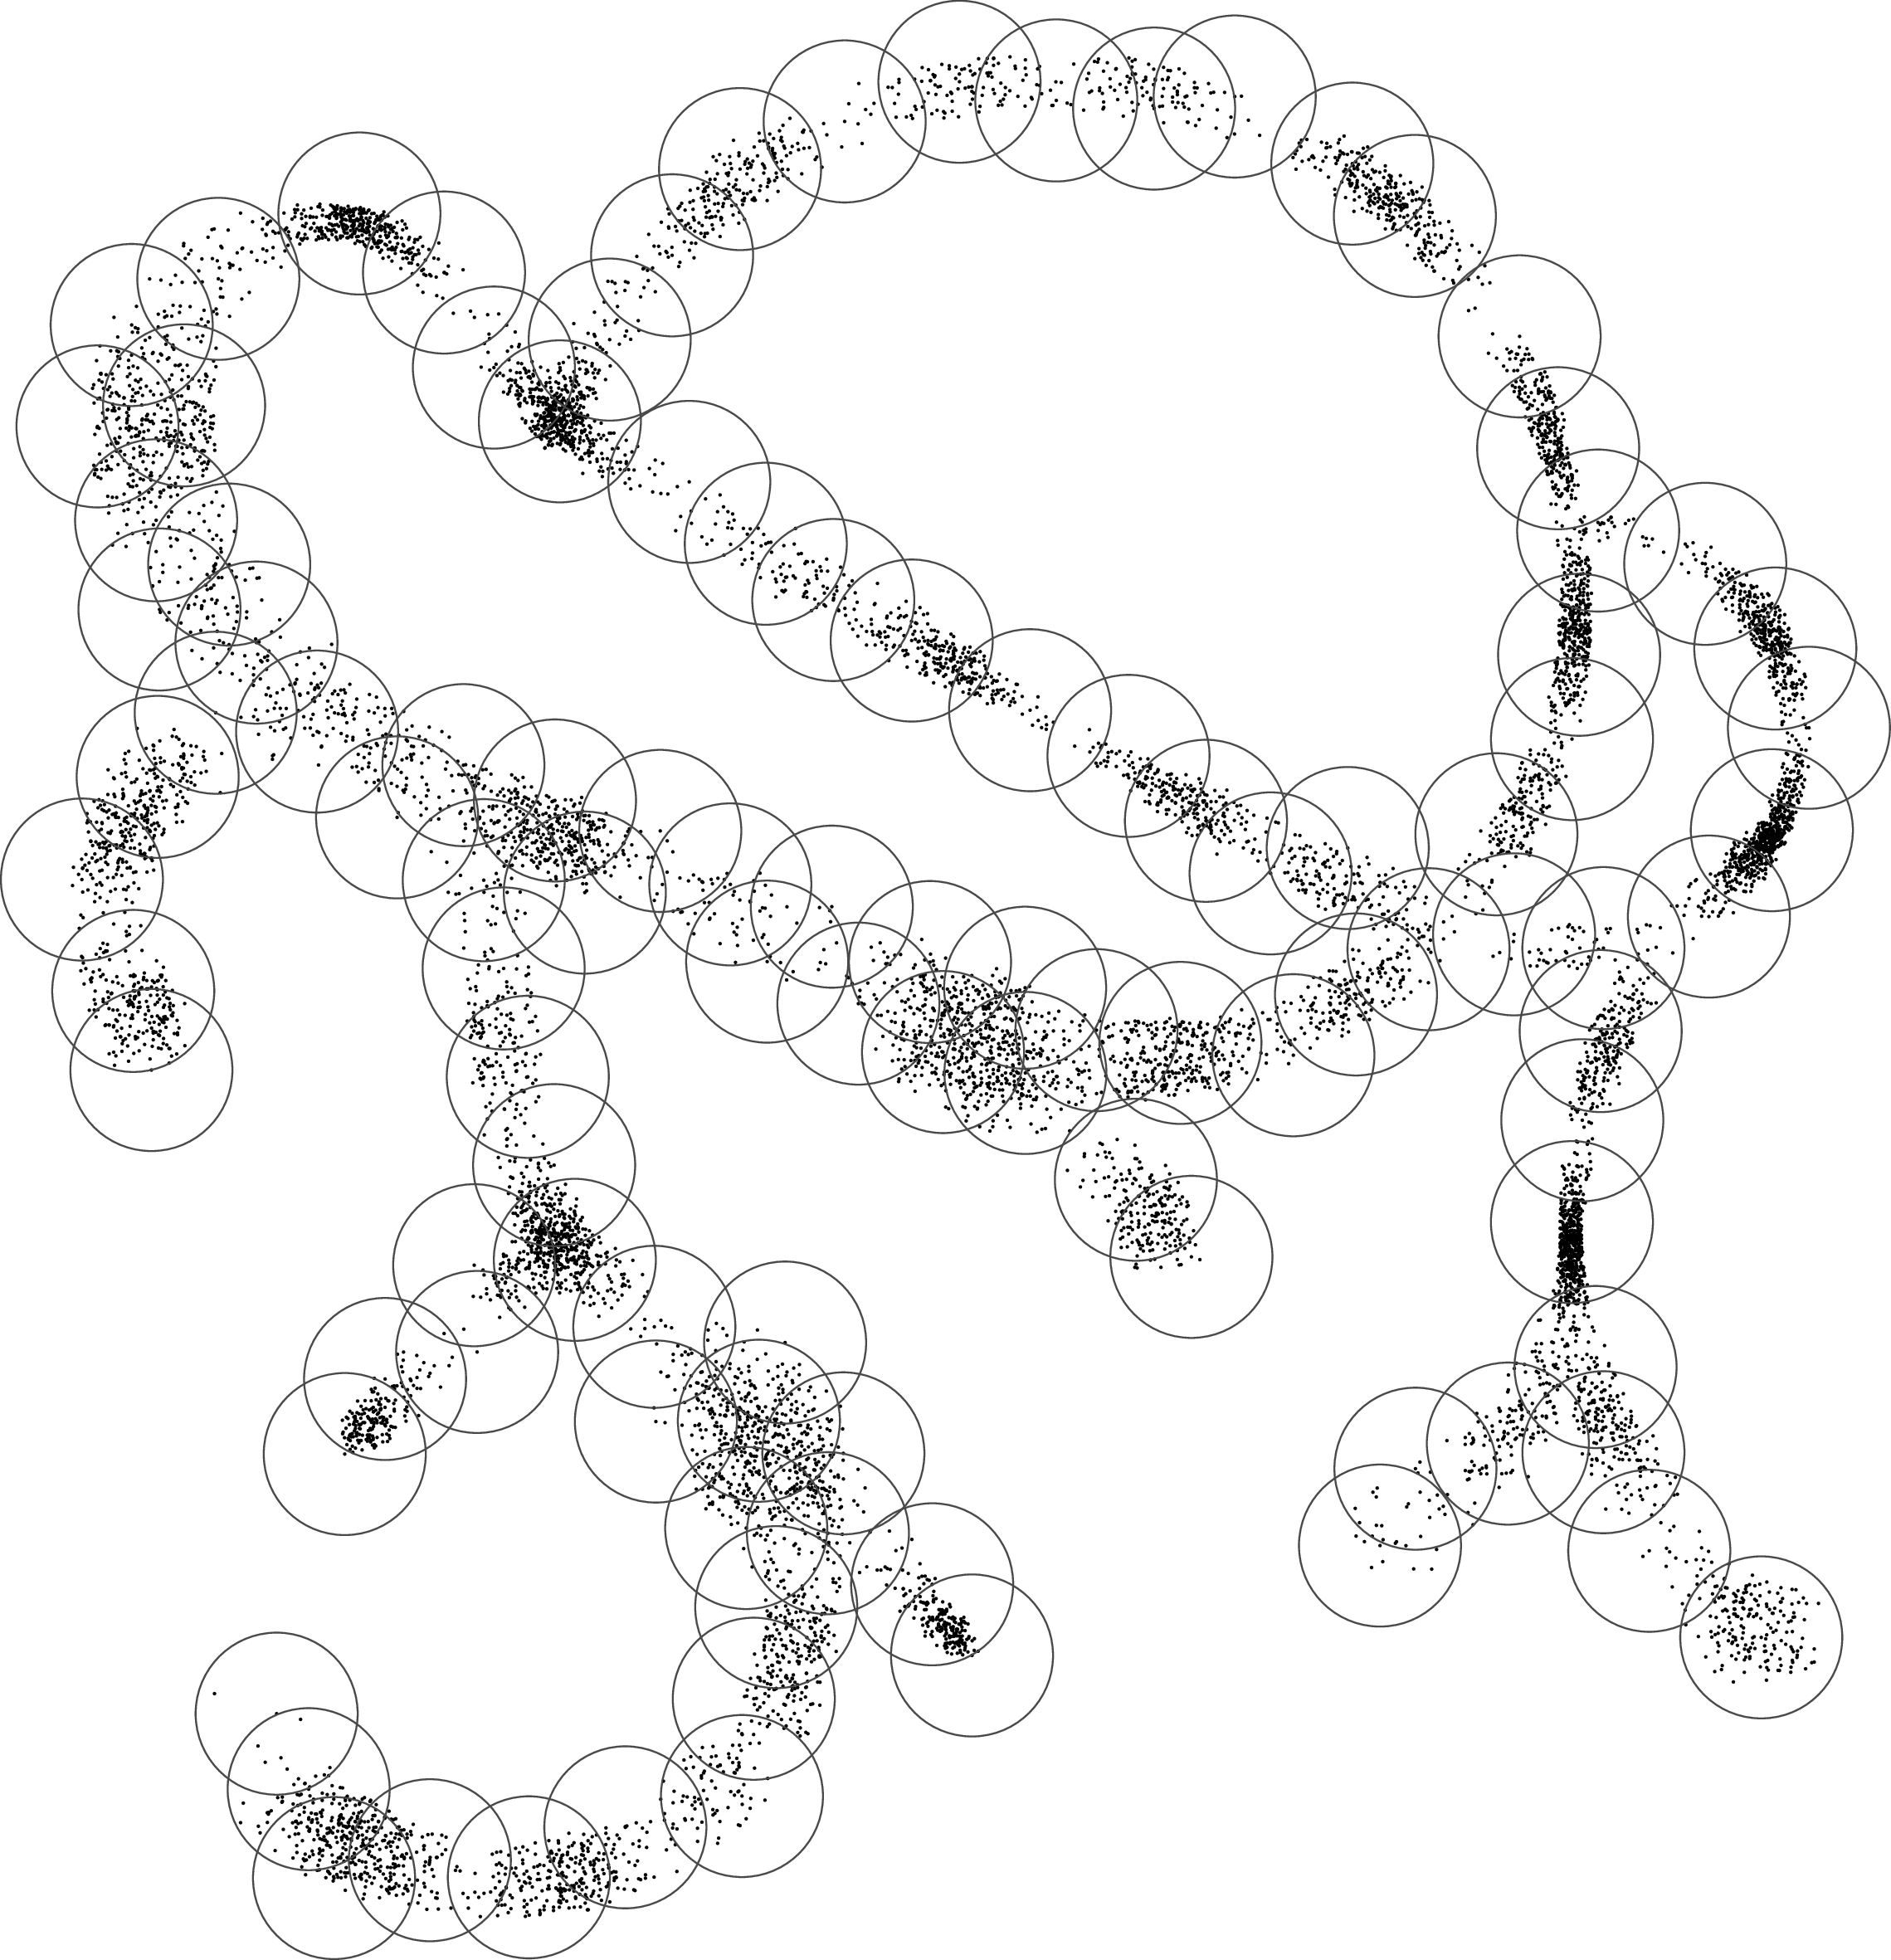
\includegraphics[width=0.8\textwidth]{assets/treepoints/treepoints2D_clusters.png}
    \caption{Cartoon depiction of points in a high-dimensional space that live close to a 1D tree-like structure. Although high-dimensional at a fine scale, at the coarser scale of covering spheres, the data cloud looks nearly 1-dimensional. Note that the cluster center generation was performed using the same algorithm used in esFragBag.}
    \label{fig:tree}
\end{figure}
More importantly, biological data sets generally do not live in low-dimensional subspaces.
Consider the instructive case of genomes along an evolutionary Tree of Life (Figure \ref{fig:tree}).
Such a tree has many branches (plus admixture merges branches back together), and looks nearly 1-dimensional locally, but is not globally.
Additionally, because of diffusion due to mutation, each of the branches is also ``thick'' (high-dimensional) when looked at closely.
%Figure 1b for illustration.
%Please look up Jinbo Xu and my work on Tree Decomposition in JACM.
% NMD: I'm familiar with TreePack, but not seeing how it's relevant.
Considering this example as a low-dimensional \textit{subspace} is incorrect.

However, the local low-dimensionality can be exploited by looking on the right scales: a coarse scale in which the tree looks 1-dimensional locally and a fine scale where the branch width matters.
We cover the tree with spheres of radius $r_c$ on the order of the branch widths; these spheres determine our clusters, and the number of them is the ``metric entropy'' of the tree \cite{tao2008product}.
Because all the points within a sphere are close to each other, they are highly redundant and can be encoded in terms of one another; thus, the metric entropy is a good approximation of the entropy of the entire database.

By the triangle inequality, to search for all points within distance $r$ of a query we need only look in nearby spheres with centers within a distance $r+r_c$ of the query.
%ref Figure 1?.
However, because the spheres have radius comparable to branch width, the tree is locally 1-dimensional on the coarse scale---we will call this the ``fractal dimension'' $d=1$ of the tree at the scale $r_c$ \cite{falconer1990fractal}.
Increasing the search radius for our coarse search only linearly increases the number of points that need to be searched in a fine search.
A similar analysis holds in the more general case.
Given a database with fractal dimension $d$ and metric entropy $k$ at the scale $r_c$, we show in the Supplemental Methods that time-complexity for similarity search with radius $r$ is
\begin{gather}
    O\Bigg(
    \underbrace{k}_{\textrm{metric entropy}} +
    \overbrace{\left|B_D(q,r)\right|}^{\textrm{output size}}
    \underbrace{\left(\frac{r+2r_c}{r}\right)^d}_{\textrm{scaling factor}}
     \Bigg) .
\end{gather}
Thus, for small fractal dimension and output size, similarity search is nearly linear in metric entropy.
Additionally, because the search only has to look at a small subset of the clusters, the clusters can be stored in compressed form, and only decompressed as needed, giving space savings that also scale with entropy.
%Similarly, using these covering spheres, the database can be stored in a 
%compressed manner (see Supplemental Methods for further details).

Real data is generally messier than the rosy picture painted here.
Sometimes the distance function is not a metric, so we lose the triangle inequality guarantee of 100\% sensitivity;
sometimes some of the points are much larger than others;
and sometimes even what counts as a point is not entirely clear without domain knowledge.
%
However, the diversity of the applications we explore in this paper demonstrate that the general scheme works for massively accelerating similarity search in a robust set of different contexts.
We expect that so long as the data set exhibits both low entropy (many items are similar to one another, which is nearly always the case when the query is a simlarity search) and low fractal dimension (the data set has some much simpler structure generating it, such as an evolutionary tree), our entropy-scaling data structure has the potential to achieve massive speedup over more naive methods and significant speedup over even other highly optimized methods.

\subsection{Metagenomics}

Metagenomics, the study of genomic data sequenced directly from environmental
samples, has recently grown in popularity.
From studies of the human gut microbiome to seawater and soil samples,
metagenomics has contributed to improved understanding of how ecosystems recover
from environmental damage~\cite{tyson2004community}, how the human gut responds 
to diet
and infection~\cite{david2014host}, and even some surprising clues as to disorders 
such as Autism Spectrum Disorder~\cite{macfabe2012short}.

Massive amounts of metagenomic reads are generated every day from 
next-generation sequencing (NGS) machines.
Overall, the rate of NGS sequencing is growing at a greater exponential rate
than computing power~\cite{loh2012compressive}.
These metagenomic reads must be stored and analyzed to do further downstream
analysis such as abundance determination (e.g. 
MetaPhlAn~\cite{segata2012metagenomic}) 
and functional characterization (e.g. PICRUSt~\cite{langille2013predictive}).
 Months of computing time are often required to process data for these novel, 
large-scale sequencing studies.
These computational challenges are at present a barrier to widespread use of 
metagenomic data throughout biotechnology, which impacts genomic medicine and 
environmental genomics~\cite{frank2008gastrointestinal}.

One approach to making metagenomic analysis tractable is to
sequence only the 16S ribosomal subunit of the microbiota, which is sufficient
to identify clades of microbes present in a sample. 
However, this approach cannot detect small functional differences between 
closely-related strains. 
In order to detect such minor functional differences, tools such as BLAST can 
be used to map metagenomic sequence data onto a database of known genome
sequences.
More recently, tools such as Kraken~\cite{wood2014kraken} have provided 
significantly faster methods for this genome mapping analysis.
This approach, however, requires a reference genome for each organism of
interest to first be identified.

Alternatively, BLASTX is widely used, both directly for analysis, as well as in 
pipelines such as MetaPhlAn~\cite{segata2012metagenomic}, to map reads to 
protein databases.
The advantage of the BLASTX approach is that complete reference genomes are not
required; BLASTX can identify homologs, particularly in the case where the
nucleotide sequence identity is low but translated protein sequence identity
is higher~\cite{turnbaugh2006obesity, kurokawa2007comparative}.
However, because BLASTX must search a protein database for possible hits for
each nucleotide read from a metagenomic sample, it is computationally intensive.
For example, \citet{mackelprang2011metagenomic} reported that using BLASTX to 
map 246
million reads against the KEGG~\cite{kanehisa2000kegg} database required 
800,000 CPU hours at a supercomputing center.
Moreover, BLASTX's run time requirements scale linearly with the size of the 
full read dataset, and each year require exponentially more runtime to process 
the exponentially growing read data. 


We present caBLASTX (compressively accelerated BLASTX), an algorithm and 
software implementation that relies on the techniques of compressive 
acceleration~\cite{loh2012compressive, daniels2013compressive} to map 
metagenomic reads onto a protein database orders of magnitude faster than 
BLASTX.

CaBLASTX is useful for two of the most common metagenomic analysis tasks. 
The first of these is mapping assembled or partially-assembled
nucleotide sequences onto a protein database. 
When these query sequences have
little in common with one another, caBLASTX maps each sequence separately. 
Each sequence is first searched against the compressed database with a 
relatively permissive E-value threshold, called coarse search. 
Any resulting hits may represent many original sequences, so these putative 
hits are expanded, and the search and alignment is refined with a less 
permissive E-value threshold, called fine search.

The second task caBLASTX can accelerate is that of mapping short nucleotide
reads (generated by next-generation sequencing technology) to a protein
database. In this instance, there is typically high coverage of the metagenomes
being sequenced, typically 30x-200x coverage. CaBLASTX takes advantage of this
redundancy
by compressing the read set as well, obtaining an additional speed gain that is
proportional to the amount of redundancy in the read data.


We tested caBLASTX on 200-400nt partially-assembled human gut microbiome
sequences, as well as on 151nt human gut microbiome reads at ~100x coverage.
For the partially-assembled sequences, we demonstrate run-time performance
approximately 10x faster than BLASTX, with negligible loss in sensitivity and
no loss in specificity. For the short reads, we demonstrate run-time
performance approximately 700x faster than BLASTX, with less than 5\% loss in
sensitivity and no loss in specificity.

CaBLASTX is a drop-in replacement for BLASTX in any pipeline.
As such, it can be used to accelerate other metagenomic analysis tools, such
as MetaPhlAn~\cite{segata2012metagenomic}.
Moreover, many of these analysis tools have, for performance reasons, required
users to construct a targeted protein database, which is a time-consuming and
possibly error-prone task.
However, caBLASTX makes it feasible to use the entire NCBI ``NR'' database for
analysis.

\subsubsection{Clustering}

CaBLASTX extends the approach of~\cite{daniels2013compressive} in order to 
cluster protein sequences.
Amino acid sequences are reduced from a 20-letter alphabet to a 4-letter
alphabet, which exposes more similarity among sequences at lower computational
cost.
This alphabet reduction can be thought of as a form of clustering; the offset 
within each of the 4 letters of the reduced alphabet is stored, so the original
sequence is recoverable (see Supplemental Methods).
CaBLASTX employs a seed-and-extend approach in order to identify similar regions
of subsequence among entries in the database (see Supplemental Methods).
This approach differs from the strict clustering described in the Data 
Structures section; in order to take advantage of the evolutionary nature of
protein sequence, \emph{subsequence} clustering is employed.
Specifically, CaBLASTX does not require that two entire protein sequences be 
similar in order to represent one in terms of the other; a similar region that 
is long enough (specifically, 40 residues at 70\% sequence identity in the 
reduced alphabet) will result in clustering of those subsequences. 
Thus, a sequence may have sub-sequences in a number of different clusters.

Given a clustering, each subsequence is represented in terms of a 
\emph{coarse sequence}, a pointer to the indices within the original sequence,
and the information required to recover the original sequence based on the
reduced alphabet.
Here, the distance function chosen, sequence identity based upon an alignment,
is decidedly not a metric.
In practice, however, as demonstrated in~\cite{daniels2013compressive} and 
here, this results in effective clustering performance with negligible loss of 
accuracy in search.

\subsubsection{Query Clustering}

Metagenomic reads are themselves nucleotide sequences, so no alphabet reduction
is performed on them directly.
Instead, metagenomic reads are compressed using the same approach as the
protein database, without the alphabet reduction step and with a number of
different parameters.
The difference scripts for metagenomic reads do not rely on the cluster offsets,
but simply store the substituted nucleotides.
Furthermore, unlike protein databases, where most typical sequences range in 
length from 100 to over 1000 amino acids, next-generation sequencing reads are 
typically short and usually of fixed length, which is known in advance.
Thus, the minimum alignment length required for a match, and the maximum
length unaligned fragment to append to a match, require different values based
on the read length.
An additional complication is that insertions and deletions from one read to
another will change the reading frame, potentially resulting in significantly
different amino acid sequences.
For this reason, query clustering requires long, \emph{ungapped} windows of high
sequence identity.
Specifically, for 202-nucleotide reads, for two sequences to cluster together,
we required a 150-nucleotide ungapped region of at least 80\% sequence identity.
Effectively, this means that the distance function for query clustering is
Hamming distance.
In the future, we may consider first translating the reads, and performing
clustering in the amino acid space (after alphabet reduction).
This would have the advantage of allowing reads with insertions or deletions
to cluster together, without causing reading-frame mismatches.
However, gapped alignment is significantly slower than ungapped alignment,
so the resulting cost of query clustering might negate speed gains.

We note that unlike the compression of the database, which can be amortized 
over future queries, the time spent clustering and compressing the queries 
cannot be amortized.
Thus, we would not refer to the query clustering as entropy-scaling, but it
still provides a practical benefit.


\subsubsection{Search}

Given a compressed protein database and a compressed query read set, search
comprises two phases.
The first, \emph{coarse search}, considers only the coarse sequences--the
representatives--resulting from compression of the protein database and the
query set.
Just as with standard BLASTX, each coarse nucleotide read is transformed into 
each of the six possible amino acid sequences that could result from it (three 
reading frames for both the sequence and its reverse complement).
Then, each of these amino acid sequences is then reduced back to a four-letter
alphabet using the same mapping as for protein database compression.
For convenience, the four-letter alphabet is represented using the standard
nucleotide bases, though this has no particular biological significance.
This is done so that the coarse search can rely on BLASTN (nucleotide BLAST) to
search these sequences against the compressed protein database.

This coarse search uses an E-value threshold that is relaxed from the one a user
specifies for the overall search, though the user can specify this coarse 
E-value threshold.
Coarse search identifies \emph{possible} hits for each query representative from
among the representative sequences in the database.
Of course, due to the reduced alphabet, some of these hits may turn out to be
poor quality when the original amino acid alphabet is considered.
Each of these coarse hits represents one or more original sequences from the
protein database; likewise, each coarse query represents one or more original
reads from the metagenomic data set.
For each coarse query representative, the set of coarse hits is used to
reconstruct all corresponding sequences from the original database by following
links to original sequence matches and applying their difference scripts.
The resulting \emph{candidates} are thus original sequences from the protein
database, in their original amino acid alphabet.
The query representative is also used to reconstruct all corresponding sequences
from the original read set.
Thus, for each coarse query representative, there is now a subset of the
metagenomic read set (the reads represented by that coarse query) and also a
subset of the protein database (the candidates).

The second phase, \emph{fine search}, uses standard BLASTX to translate each
of these reads associated with a coarse query representative and search for
hits only in the subset of the database comprising the candidates.
This fine search phase relies on a user-specified E-value threshold (defaulting
to BLASTX's default of 10) to filter hits.
To ensure that E-value calculation is correct, BLASTX uses a corrected database
size which is the size of the original, uncompressed protein database.

\subsubsection{Benchmarking}

To evaluate the run-time performance of caBLASTX, we tested it against
BLASTX as well as RapSearch2~\cite{zhao2012rapsearch2} and
Diamond~\cite{buchfink2014fast}.
BLASTX is often used to align assemblies thought to be exons to a protein
database, in which case metagenomic reads have already been assembled.
In this instance, the query-side compression of caBLASTX is not applicable, so
the performance gains are more modest.
We benchmarked caBLASTX vs. BLASTX on a dataset consisting of 22,778 assemblies
from human gut microbiota, 3.1 megabases in total, searching against the NCBI's
``NR'' non-redundant protein database from September, 2014.
The running time of BLASTX was 3235 minutes, compared to 123 minutes for caBLASTX, a speedup of 26.3.

When aligning unassembled next-generation sequencing reads to a protein 
database, the
query-side clustering aspect of caBLASTX becomes applicable.
We benchmarked caBLASTX against BLASTX on a set of 100,000
next-generation sequencing reads each of length 202 nucleotides from a human 
fecal dataset (SRR059854) from the
Human Microbiome Project~\cite{turnbaugh2007human}.
We filtered out reads starting or ending with 10 or more no-calls ('N').
The running time for BLASTX was 14,423 minutes, 
while caBLASTX took 21 minutes, a speedup of 673.
Results appear in Table~\ref{mgbench}.

\begin{table}
\caption{Comparison of caBLASTX and BLASTX running time and accuracy.\label{mgbench}}
\begin{tabular}{ccccc}
\hline
dataset & BLASTX (s) & caBLASTX  (s) & speedup & accuracy\\
\hline
assemblies & 3235 & 123 & 26.3x & 99.2\%\\
\hline
NGS reads & 14423 & 21 & 673x & 95.7\%\\
\hline
\end{tabular}
\end{table}



\subsubsection{Validation}

In order to validate caBLASTX's accuracy, we treated BLASTX as a gold standard. 
Since caBLASTX accelerates BLASTX
using entropy-scaling techniques, false positives with respect to BLASTX should 
not be possible, but false negatives certainly are.
We evaluated the hits from BLASTX and caBLASTX on the same human gut
assemblies and raw reads used for benchmarking, in order to evaluate the accuracy when
query-side compression is not used.
As false positive hits with respect to BLASTX are not possible, we report as 
accuracy the fraction of BLASTX hits that are also returned by caBLASTX.
We note that due to query-side compression, the output order from caBLASTX 
typically does not match that of BLASTX.
As show in Table~\ref{mgbench}, on the metagenomic assemblies, where query-side 
compression was not performed, caBLASTX achieves 99.2\% accuracy, while on the 
raw reads, caBLASTX achieves 95.7\% accuracy.


\subsection{High-throughput Drug Screening}

In the field of drug discovery and drug repurposing, prediction of biologically 
active compounds is a critical task. 
Computational high-throughput screening can eliminate many compounds from 
wet-lab consideration, but even this screening can be computationally 
intensive, and thus time-consuming.
PubChem~\cite{bolton2008pubchem} is a repository of molecular compound 
structures, 
which has grown exponentially since 2008 (Figure~\ref{pubchemdata}). 
In October, 2013, PubChem contained roughly 47 million molecular structures; 
in December, 2014 it contains 61.3 million structures.

We introduce a framework for clustering molecular databases that use the 
popular SDF molecular structure format, such as PubChem, and for searching for 
similar molecular structures in compressed space.
We designed this compression and search framework around one of the standard 
techniques for high-throughput screening of potential drug compounds, the use 
of maximum common subgraph (MCS) to identify similar motifs among molecules \cite{cao2008maximum, rahman2009small}.
Using an entropy-scaling approach, our new software Ammolite is able to achieve \hl{?????}.
As intimated above, not only is Ammolite a practical tool ready for use by biochemists, but its results also demonstrate the scalability of entropy scaling methods as databases grow.

In developing Ammolite, we augmented the entropy-scaling data structure by introducing different but related distance functions for the coarse versus fine search.
For the fine search, 
we implemented a variant of the maximum common subgraph (MCS) algorithm, known as 
\emph{flexible} maximum
common subgraph (fMCS), as detailed by Cao, et al.~\cite{cao2008maximum}.

For the coarse search, however, we first project the space of small molecules onto a subspace by removing nodes and edges that do not particiapte in simple cycles.
Clusters are exactly pre-images of of this projection operator (i.e. all molecules that are isomorphic after simplification form a cluster).
Coarse search is performed using fMCS on this much smaller projection subspace, greatly increasing speed.

%Many existing MCS-based tools, such as SMSD~\cite{rahman2009small} and 
%fmcsR~\cite{cao2008maximum} compute the maximum common subgraph on fully 
%labeled graphs; 
%vertices are labeled with chemical elements, and edges are labeled with bond 
%types (such as single or double bonds).
%The `f' in fmcsR, which stands for ``flexible,'' indicates that some bounded 
%number of vertex or edge label mismatches are permitted, at significant 
%computational cost.
\hl{Benchmarking paragraph(s)}

\hl{Validation paragraph(s)}

\subsection{Protein Structure Search}

The relationship between protein structure and function has been a subject of intense study for decades,
and this strong link has been used for the fruitful prediction of function from structure \cite{hegyi1999relationship}.
To wit, given a protein of solved (or predicted) structure but unknown function, the efficient identification
of structurally similar proteins in the Protein Data Bank is critical to function prediction.
Relatedly, finding structural neighbors can also give insight into the evolutionary origins of proteins of interest.

One approach to finding structural neighbors is to attempt to align the query protein to all the entries in the Protein Data Bank (PDB) using a structural aligner (e.g. STRUCTAL \cite{subbiah1993structural} or ICE \cite{shindyalov1998protein}).
However, performing a full alignment against every entry in the PDB is prohibitively expensive, especially as the database grows.
Alternately, the approach we use here is the one introduced by FragBag~\cite{budowski2010fragbag}, which describes each protein as a
``bag of fragments,'' where each fragment is a small structural motif.
By directly applying our entropy scaling data structure without any additional augmentation, esFragBag (entropy scaling FragBag) is able to achieve a 2-30x speedup of FragBag with less than 0.2\% loss in sensitivity and no loss in specificity.

For this last example, we intentionally approached the application of entropy-scaling data structures to FragBag in a blind manner,
without using any domain-specific knowledge.
Instead, we used the very same representation (bag of fragments) and distance functions (Euclidean and cosine distances)
as FragBag, a greedy k-centers algorithm, and vector difference to generate the clustered representation.
Note that this is in stark contrast to caBlastX and Ammolite, which both exploited domain knowledge to further improve performance.
Thus, esFragBag only involves grafting new database generation and similarity search functions onto an existing codebase.
Although using similar techniques to exploit domain specific knowledge as in caBlastX and Ammolite might result in greater speedup, esFragBag here is explored as a proof-of-concept to analyze the performance of a the entropy-scaling data structure alone.

We explored the increases in speed resulting from applying the entropy-scaling data structure, for both Euclidean and cosine distances (Figure \ref{fig:fragbag}).
Naturally, as search radii increases, the coarse search expands to encompass the entire database; to fully explore parameters, we made certain to increase search radii until the acceleration effect entirely disappeared.
Additionally, we explored the effect of using different maximum cluster radii and several different query proteins.

For cosine distance, we generated databases with maximum cluster radii of 0.1, 0.2, 0.3, 0.4, and 0.5.
Then, for each query protein from the set \{\texttt{4rhv}, \texttt{1ake}, \texttt{1bmf}, \texttt{1rbp}, \texttt{1b7t}\}, we ran both naive and accelerated similarity searches with radii of $0.02i \forall i \in \{0,\ldots,49\}$.
This was repeated 5 times for each measurement, and the ratio of average accelerated vs naive times is shown in Figure \ref{fig:fragbag_cosine}.

For euclidean distance, we generated databases with maximum cluster radii of 10, 20, 25, 50, and 100.
Again, for each query protein drawn from the same set, we compared the average over 5 runs of the ratio of average accelerated vs naive times (Figure \ref{fig:fragbag_euclid}.

As expected, the acceleration is highly dependent on both the search radius $r$ and the maximum cluster radius $r_c$.
Additionally, the query protein also makes a major difference in the results.
We suspect that this is due to the geometry of protein fragment frequency space being very ``spiky'' and ``star-like''.
Proteins that are near the core (and thus similar to many other proteins) show very little acceleration when our data structure is used because the majority of the database is nearby, whereas proteins in the periphery have fewer neighbors and are thus found much more quickly.
Changing the maximum cluster radius effectively makes more proteins peripheral proteins, but at the cost of overall acceleration.

Naturally, as the search radius expands, it quickly becomes necessary to compare against nearly the entire database, destroying any acceleration.
For the cosine space in particular, note that the maximum distance between any two points is $1$, so once the coarse search radius of $r+r_c >= 1.0$, there cannot ever be any acceleration as the fine search encompasses the entire database.
Similarly, once the coarse search encompasses all (or nearly all) the clusters in Euclidean space, the acceleration diminishes to 1x, and the overhead costs make the entropy scaling data structure perform worse than a naive search.
However, as we are most interested in proteins that are very similar to the query, the low-radius behavior is of primary interest.
In the low-radius regime, esFragBag demonstrates varying though substantial acceleration (2x-30x) over FragBag.

Additionally, it is instructive to note that because of the very different geometries of euclidean vs cosine space, acceleration varies tremendously for some proteins, such as \texttt{4rhv} and \texttt{1bmf}, which display nearly opposite behaviors.
Whereas there is nearly 30x acceleration for \texttt{4rhv} in cosine space for low radius, and the same for \texttt{1bmf} in euclidean space, neither achieves better than $\sim$ 2.5x acceleration in the other space.

\begin{figure}[tbp]
    \centering
    \begin{subfigure}[b]{0.40\textwidth}
        \caption{Cosine distance}
        \label{fig:fragbag_cosine}
        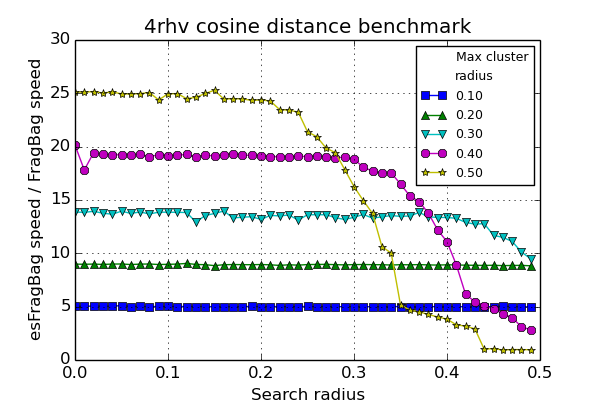
\includegraphics[width=1\textwidth]{assets/4rhv_cosine.png}
    \end{subfigure}%
    \begin{subfigure}[b]{0.40\textwidth}
        \caption{Euclidean distance}
        \label{fig:fragbag_euclid}
        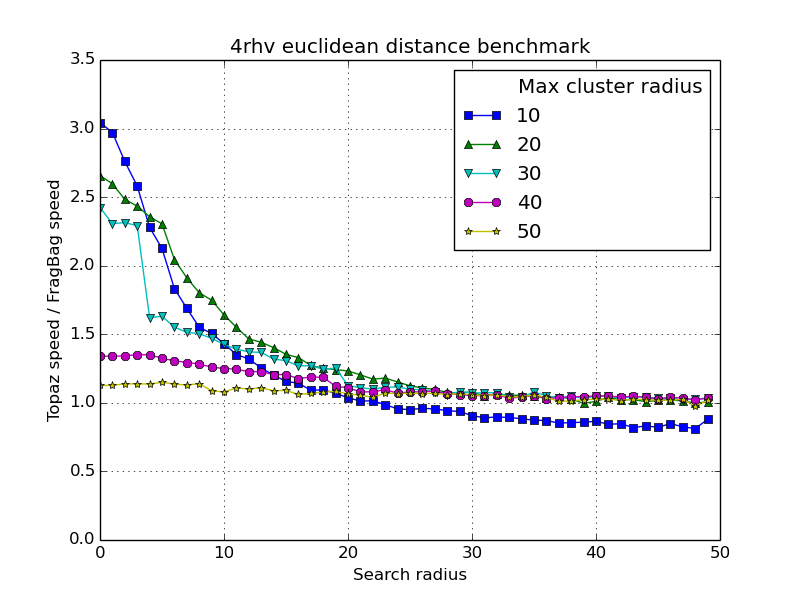
\includegraphics[width=1\textwidth]{assets/4rhv_euclid.png}
    \end{subfigure}
    \begin{subfigure}[b]{0.40\textwidth}
        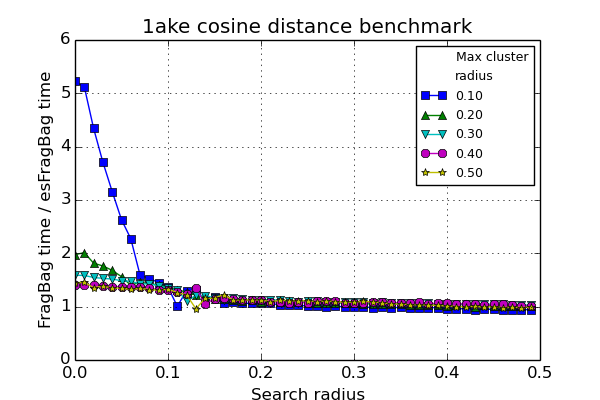
\includegraphics[width=1\textwidth]{assets/1ake_cosine.png}
        %\caption{}
    \end{subfigure}%
    \begin{subfigure}[b]{0.40\textwidth}
        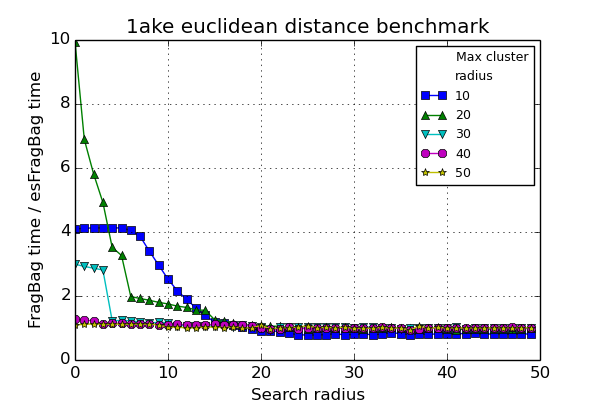
\includegraphics[width=1\textwidth]{assets/1ake_euclid.png}
        %\caption{}
    \end{subfigure}
    \begin{subfigure}[b]{0.40\textwidth}
        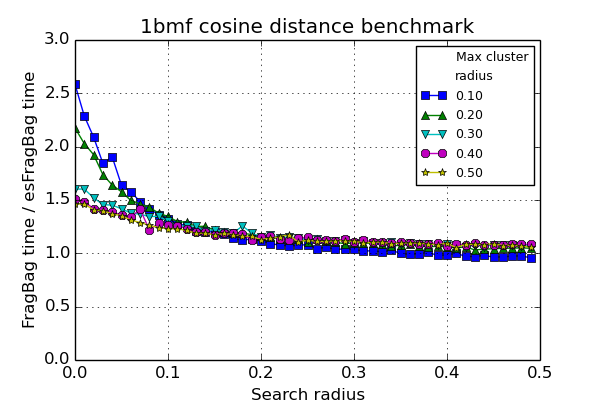
\includegraphics[width=1\textwidth]{assets/1bmf_cosine.png}
        %\caption{}
    \end{subfigure}%
    \begin{subfigure}[b]{0.40\textwidth}
        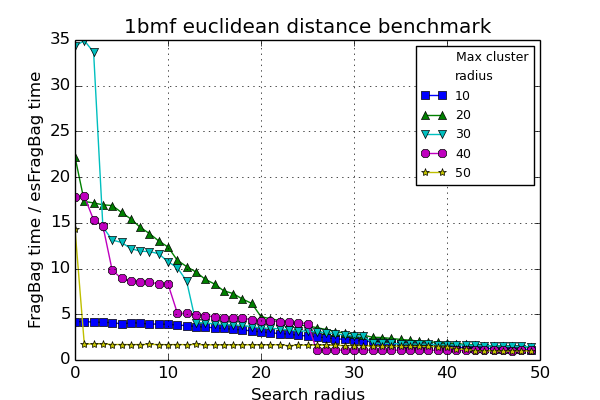
\includegraphics[width=1\textwidth]{assets/1bmf_euclid.png}
        %\caption{}
    \end{subfigure}
    \begin{subfigure}[b]{0.40\textwidth}
        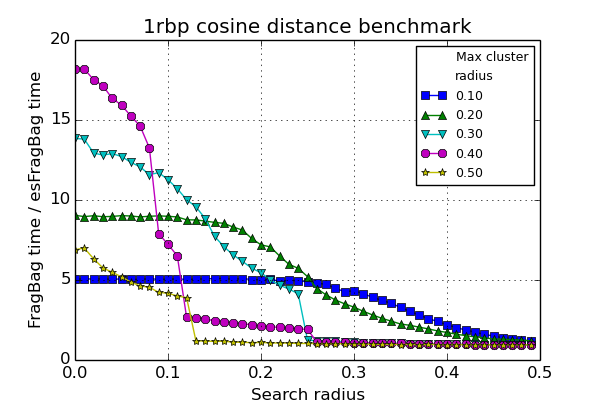
\includegraphics[width=1\textwidth]{assets/1rbp_cosine.png}
        %\caption{}
    \end{subfigure}%
    \begin{subfigure}[b]{0.40\textwidth}
        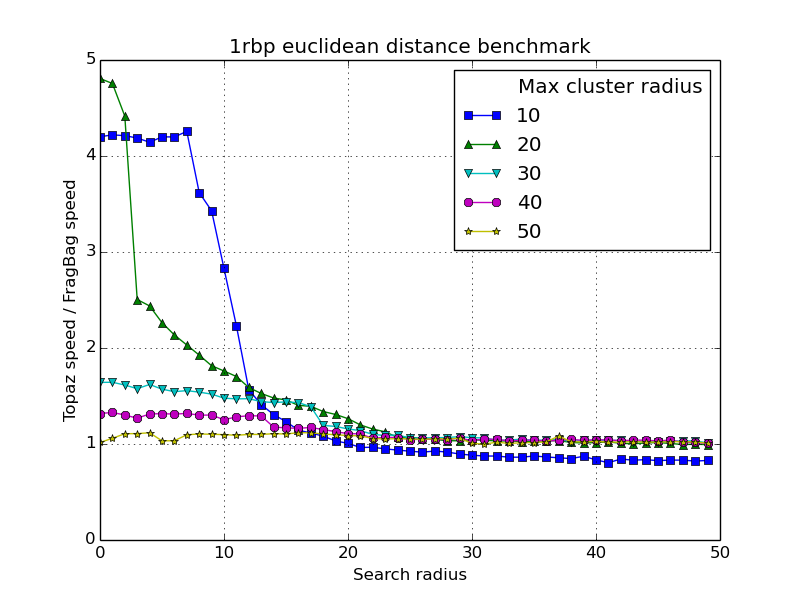
\includegraphics[width=1\textwidth]{assets/1rbp_euclid.png}
        %\caption{}
    \end{subfigure}
    \caption{FragBag benchmarking data. (a) Cosine distance gives on the whole better acceleration, but results in only $>99.8\%$ sensitivity, whereas (b) Euclidean distance as a metric is guaranteed by the Triangle Inequality to get $100\%$ sensitivity.}
    \label{fig:fragbag}
\end{figure}

Finally, while Euclidean distance is a metric---for which the triangle inequality guarantees 100\% sensitivity---cosine distance is not.
Empirically, however, for all of the queries we performed, we achieve $> 99.8\%$ sensitivity (Table \ref{tab:fragbag_cosine_sensitivity}).
%Full results for each data point can be found in supplementary data files.

\begin{table}
    \centering
    \caption{Average sensitivity of esFragBag compared to FragBag when using cosine distance for the trials described in Figure \ref{fig:fragbag_cosine}. This table averages the sensitivities for each choice of search radii $\{0, 0.01, \ldots, 0.49\}$. (NB: no analogous table is given for euclidean distance as the Triangle Inequality ensures perfect recall).}
    \label{tab:fragbag_cosine_sensitivity}
    \begin{tabular}{|c|cccc|}
        \hline
        \backslashbox{Cluster radii}{Query protein}  & 4rhv & 1ake & 1bmf & 1rbp \\
        \hline
        0.10  & 1  & 0.999840     & 0.998490 & 0.999950  \\
        0.20  & 1  & 0.999918     & 0.999001 & 0.999978  \\
        0.30  & 1  & 0.999926     & 0.999649 & 1  \\
        0.40  & 1  & 0.999974     & 0.999796 & 1  \\
        0.50  & 1  & 0.999984     & 0.999934 & 1  \\
        \hline
    \end{tabular}
\end{table}

\section{Discussion}

We have introduced a data structure for accelerating approximate search, and
demonstrated its effectiveness in three distinct areas of computational
molecular biology.
This data structure provably scales almost linearly with entropy of the 
database, allowing search on large data sets to scale even as these data sets
grow exponentially.
We provide open-source software for all three areas: caBlastX for metagenomic analysis,
Ammolite for small-molecule structure search, and esFragBag for protein structure search.
In the case of metagenomic analysis, caBLASTX also compares favorably to recent 
search tools that outperform BLASTX.

In this work, we have not focused on the space-saving compression that is
possible with entropy-scaling data structures, but rather on the run-time
acceleration of approximate search.
However, particularly in the case of metagenomic analysis, the collection of 
read data presents a problem for storage and transfer, as well as analysis.

\section{Methods}
\subsection{Cablastx}

\subsection{Ammolite}
Our clustering approach relies on structural similarity.
In order to more effectively group molecules based on structural motifs,
each molecule is \emph{simplified} by removing nodes and edges that do not
participate in simple cycles.
Clusters are formed of molecules that are isomorphic after this simplification
step.
Each cluster can then be represented by a single molecular structure, along 
with pointers to \emph{difference sets} between that structure and each of the 
full molecules it represents.
The difference set contains the nodes and edges that were removed in the 
simplification step.

We implemented a variant of a maximum common subgraph (MCS) algorithm, known as 
\emph{flexible} maximum
common subgraph (fMCS), as detailed by Cao, et al.~\cite{cao2008maximum}.
Our implementation allows a user to specify whether any atom mismatches or 
bond-type mismatches should be 
allowed in the maximum common subgraph of two molecules.
If zero mismatches are allowed, fMCS is just MCS.
The distance function used currently is based on the overlap coefficient 
defined as $d(G_1,G_2) = 1 - \frac{ |mcs(G_1,G_2)| }{min(|G_1|,|G_2|)}$. This function, unlike 
the graph distance function  ~\cite{bunke1998graph}, is not a metric. However it does account for
situations where a large molecule contains a smaller molecule which is important in practice.

As in~\cite{loh2012compressive}, our compression-accelerated search approach 
relies on a two-stage process.
First, a \emph{coarse} search is performed in compressed space, by searching 
the coarse database.
The query molecule is simplified in exactly the same manner as 
the molecular database during clustering, and this transformed query graph is 
matched against the coarse database.
To preserve sensitivity, this coarse search is performed with a permissive 
similarity score.
The idea behind coarse search is to identify \emph{possible} hits.


Any possible hits--molecular graphs from the coarse database whose MCS to 
the transformed query molecule was within the similarity score threshold--are 
then reconstructed, by following
pointers to the removed atom and bond information, and recreating the 
original molecules.

Next, the \emph{fine search} is performed against these decompressed possible 
hits.
Fine search is performed using MCS or fMCS, with user-defined parameters for 
bond and atom mismatches and similarity-score threshold.


\subsection{esFragBag}
In FragBag, the bag of fragments is essentially
a term frequency vector representing the number of occurrences of each structural motif within the protein.
While FragBag does not generate structural alignments the way standard aligners do, it provides an excellent
filter for computing proteins that are likely to have close alignments; those alignments could then be computed
with a standard aligner.
FragBag's accuracy has been reported as comparable to structural aligners such as STRUCTAL and
ICE.
FragBag is already quite fast, much faster than these standard aligners, but also importantly for us
FragBag turns out to be very amenable to acceleration using an entropy-scaling data structure because much of the computation is spent in doing a similarity search on a frequency vector.

For the cluster generation, we used a randomized greedy 2-pass approach.
First, all proteins in the Protein Data Bank were randomly ordered.
Then in the first pass, proteins were selected as cluster centers if and only if they were not within a user-specified Euclidean distance $r_c$ from an existing center (i.e. the first protein is always selected, and the second if further away than $r_c$ from the first, etc.).
Recall that this generation of cluster centers is the same as the one used to generate covering spheres in Figure \ref{fig:tree};
the covering spheres were overlapping, but we trivially assign every protein uniquely to a single cluster by assigning to the nearest cluster center in the second pass.

Similarity search here is performed exactly as described in the data structure section, with no modifications.
For a given search query $q$ and search radius $r$,
\begin{itemize}
    \item A coarse search is used to find all cluster centers within distance $r+r_c$ of $q$.
    \item All corresponding clusters were unioned into a set $F$.
    \item A fine search was performed over the set $F$ to find all proteins within distance $r$ of $q$.
\end{itemize}

\section{Author Contributions}
Y.W.Y., N.M.D. and B.B. conceived the project.
Y.W.Y. and B.B. developed the theoretical analyses, with help from N.M.D.
N.M.D. implemented and benchmarked Cablastx.
D.C.D. implemented and benchmarked Ammolite, with help from N.M.D.
Y.W.Y. applied the entropy-scaling data structure to accelerate FragBag, with help from N.M.D.
B.B. guided all research and provided critical advice on the study.
Y.W.Y., N.M.D. and B.B. wrote the manuscript.

\section{Acknowledgments}
Y.W.Y. is supported by a Hertz Foundation fellowship.
N.M.D. and B.B. are supported by NIH GM108348.
We thank Andrew Gallant for his implementation of Fragbag.

\bibliographystyle{model5-names-noitalic}
%\bibliographystyle{plain}
\bibliography{main}

\end{document}

